%%%%%%%%%%
% Required package and library
\usepackage{tikz}
\usetikzlibrary{calc}
%%%%%%%%%%

\newcommand{\sSFR}{ {\rm sSFR}^{-1}\!\!\!-\!{\rm ZR} }
\def\alpMZR{\alpha=0.0}
\def\alpFMR{\alpha\neq0.0}

\definecolor{Mycolor1}{HTML}{A93F53}
\definecolor{Mycolor2}{HTML}{3DA6A1}
\definecolor{Mycolor3}{HTML}{FEFB39}

\def\colorOne{Mycolor1!60!red!60}
\def\colorTwo{Mycolor2!60!white}
\def\colorThree{Mycolor3!70!white}

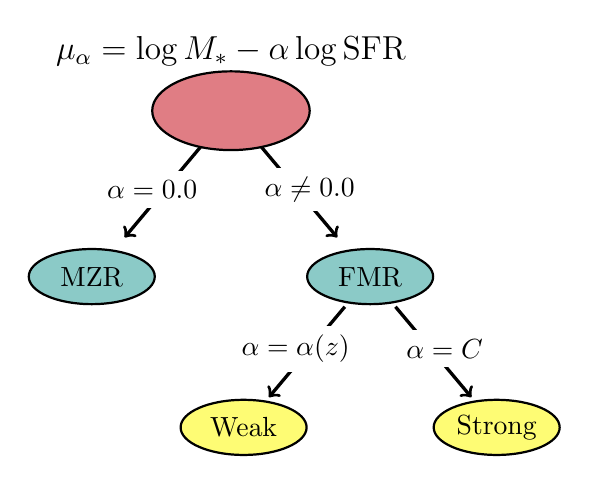
\begin{tikzpicture}
    \foreach \angle\name\alpVal\x in {-40/MZR/$\alpMZR$/-1,40/FMR/$\alpFMR$/1} {
        \begin{scope}[rotate around={\angle:(0,0)}]
            \draw[->,very thick] (0,0) -- (0,-2.1);
            \coordinate (\name) at (0,-2.75);
        \end{scope}
        \draw[fill=\colorTwo, thick] (\name) ellipse (0.8 and 0.35) node[] {\name};
        \node[fill=white] at (\x,-1) {\alpVal};
    }

    \draw[ fill=\colorOne, thick ] (0,0) ellipse (1 and 0.5) node[] {$\muZR$}; 
    \node[] at (0,0.75) {\large $\mu_{\alpha} = \log M_* - \alpha\log {\rm SFR}$};

    \foreach \angle\name\label in {-40/LFMR/Weak,40/aFMR/Strong} {
        \begin{scope}[rotate around={\angle:(FMR)}]
            \draw[->,very thick] ($(FMR) - (0,0.5)$) to ($(FMR) - (0,2)$);
             \coordinate (\name) at ($(FMR) - (0,2.5)$);
        \end{scope}
        \draw[fill=\colorThree, thick] (\name) ellipse (0.8 and 0.35) node[] {\label};
    }
    
    \node[fill=white] at ($(LFMR) + (0.66,1)$) {$\alpha=\alpha(z)$};
    \node[fill=white] at ($(aFMR) + (-0.66,1)$) {$\alpha=C$};
\end{tikzpicture}